\begin{figure}
\centering

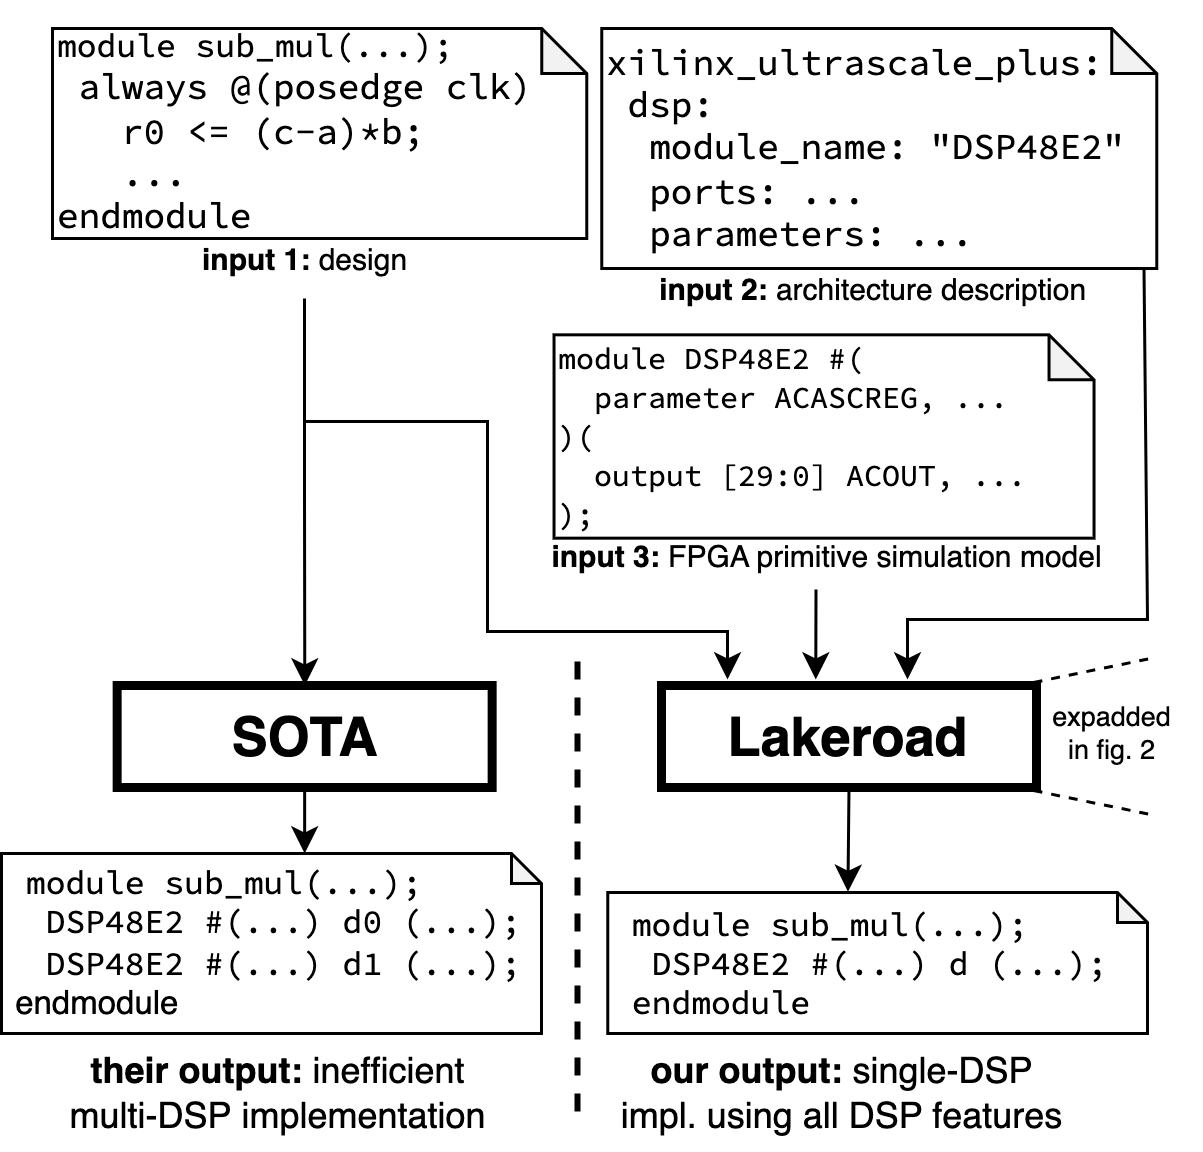
\includegraphics[width=0.91\columnwidth]{assets/lakeroad-firstpage.drawio.png}

% \vspace{3mm}
% \resizebox{0.4\textwidth}{!}{
% \begin{tabular}{cc|c|c}
% Design& \# Stages &  SOTA& \lr \\ \hline
% \texttt{((d+a)*b)|c}& 1 &2 DSP, 18 LUT & 1 DSP  \\
% \texttt{((d+a)*b)\textasciicircum{}c} & 1 & 2 DSP, 18 LUT  & 1 DSP \\
% \texttt{((d-a)*b)|c} & 2 & 2 DSP, 18 LUT & 1 DSP \\
% \texttt{((d-a)*b)\textasciicircum{}c} &  2          & 2 DSP, 18 LUT & 1 DSP \\
% \texttt{((d+a)*b)\&c}& 2 & 2 DSP, 18 LUT & 1 DSP \\
% \end{tabular}}
\vspace{-3mm}
\caption{
% Mapping a simple design to
%   Xilinx UltraScale+ FPGAs with both
%   the state of the art (SOTA)
%   hardware synthesis tool for Xilinx
%   and \lr.
Even given a simple input
  design (input 1),
  the state-of-the-art (SOTA)
  hardware synthesis tool
  for Xilinx FPGAs
  frequently
  fails to efficiently use 
  programmable primitives
  like DSPs.
\lr,
  on the other hand,
  can utilize all features
  of programmable primitives
  given just a short description
  of an FPGA architecture (input 2)
  and the vendor-provided 
  simulation models
  of the primitive (input 3).\tighten
}
\label{fig:firstpage}

\vspace{-5mm}
\end{figure}
